\documentclass[dvisvgm,tikz]{standalone}

\usepackage{amsmath}
\usepackage{mathpazo}
\usepackage[utf8]{inputenc}
\usepackage{graphics}
\usepackage[colorlinks,urlcolor=blue]{hyperref}
\usepackage{standalone}
\usepackage{svg}
\usepackage{tikz}

\usetikzlibrary{arrows.meta,decorations.pathreplacing,calligraphy}
\special{background White}

\begin{document}
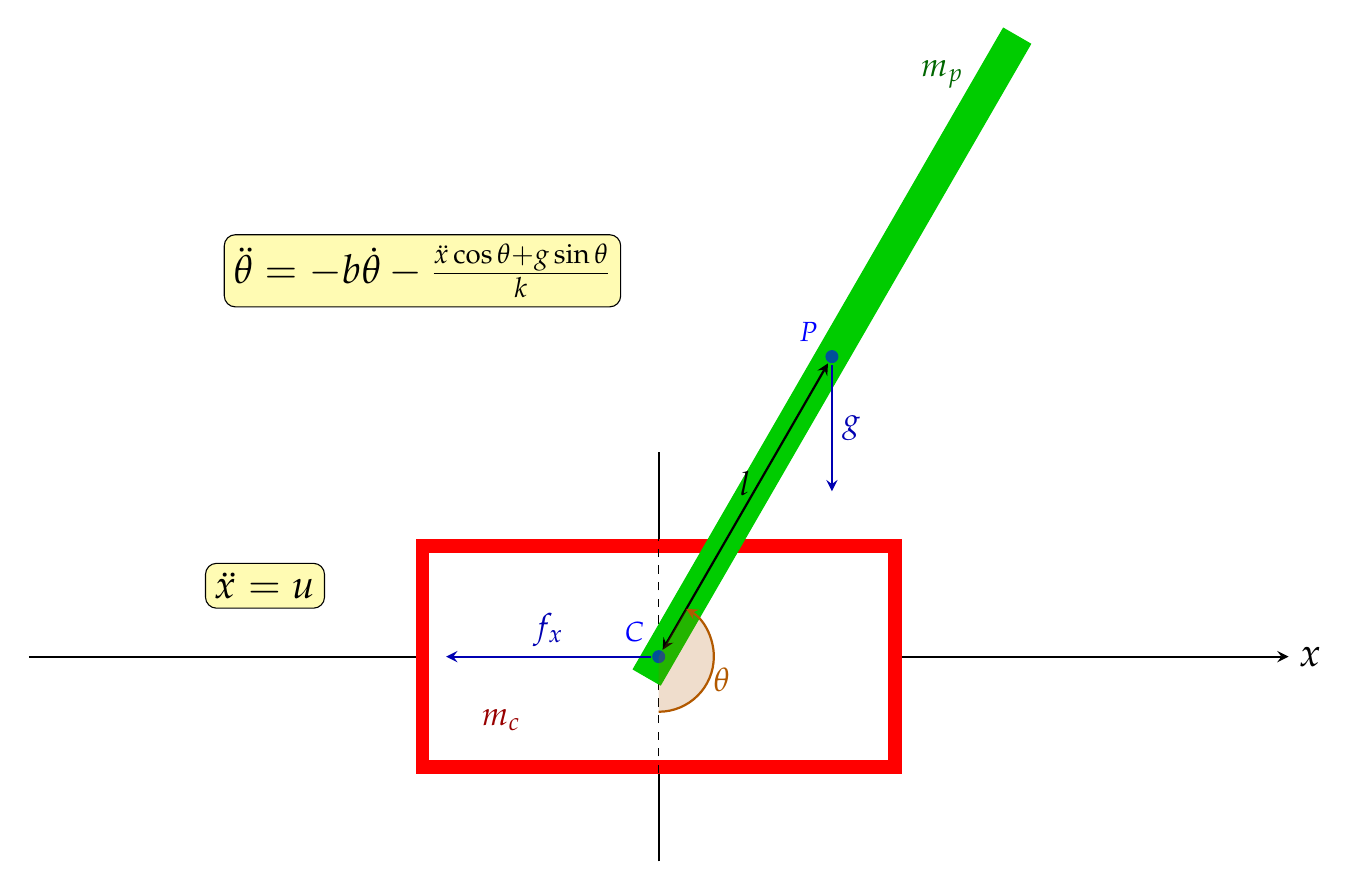
\begin{tikzpicture}[>=stealth]
    % world
    \draw[->, thick] (-1,3.1) -- (15,3.1) node[right] {\Large $x$};
    \draw[-, thick] (7,0.5) -- (7,5.7);

    % hull
    \filldraw[red!100!black, fill=white, line width=5] (4.0,1.7) rectangle (10.0,4.5);

    % y axis help
    \draw[-, dashed] (7,1.2) -- (7,5.0);

    % stick
    \begin{scope}[rotate around={150:(7, 3.1)}]
        \filldraw[green!80!black, fill=green!80!black] (6.8, 3.4) rectangle (7.2, -6);

        % C
        \node[circle, fill=blue, opacity=0.6, scale=0.5, label={above left:{\textcolor{blue}{$C$}}}] at (7, 3.1) {};

        % P
        \node[circle, fill=blue, opacity=0.6, scale=0.5, label={above left:{\textcolor{blue}{$P$}}}] at (7, -1.3) {};

        % l
        \draw[<->, thick, black] (7,3) -- (7, -1.2) node[midway,above] {\large $l$};
    \end{scope}

    % f_x
    \draw[<-, thick, blue!70!black] (4.3,3.1) -- (6.9, 3.1) node[midway,above] {\large $f_x$};

    % g
    \draw[->, thick, blue!70!black] (9.2, 6.81) -- (9.2, 5.2) node[midway,right] {\large $g$};

    % \theta
    \draw[->, thick, orange!70!black] (7, 2.4) arc [start angle=-90, end angle=60, radius=0.7];
    \fill[->, opacity=0.2, orange!70!black] (7, 3.1) -- (7, 2.4) arc [start angle=-90, end angle=60, radius=0.7];
    \draw[thick, orange!70!black] (7.8, 2.8) node {\large $\theta$};

    % m_C
    \draw[red!60!black] (5, 2.3) node {\large $m_c$};

    % m_P
    \draw[green!40!black] (10.6, 10.5) node {\large $m_p$};

    % formula
    \draw (4,8) node[fill=yellow!30, draw, rounded corners] {\Large $\ddot{\theta} = -b\dot{\theta} -\frac{\ddot{x} \cos \theta + g \sin \theta}{k}$};
    \draw (2,4) node[fill=yellow!30, draw, rounded corners] {\Large $\ddot{x} = u$};
\end{tikzpicture}
\end{document}
